% ****** Start of file apssamp.tex ******
%
%   This file is part of the APS files in the REVTeX 4.2 distribution.
%   Version 4.2a of REVTeX, December 2014
%
%   Copyright (c) 2014 The American Physical Society.
%
%   See the REVTeX 4 README file for restrictions and more information.
%
% TeX'ing this file requires that you have AMS-LaTeX 2.0 installed
% as well as the rest of the prerequisites for REVTeX 4.2
%
% See the REVTeX 4 README file
% It also requires running BibTeX. The commands are as follows:
%
%  1)  latex apssamp.tex
%  2)  bibtex apssamp
%  3)  latex apssamp.tex
%  4)  latex apssamp.tex
%
\documentclass[%
 reprint,
superscriptaddress,
%groupedaddress,
%unsortedaddress,
%runinaddress,
%frontmatterverbose, 
%preprint,
%preprintnumbers,
%nofootinbib,
%nobibnotes,
%bibnotes,
 amsmath,amssymb,
 aps,
%pra,
%prb,
%rmp,
%prstab,
%prstper,
%floatfix,
]{revtex4-2}

\usepackage{graphicx}% Include figure files
\usepackage{dcolumn}% Align table columns on decimal point
\usepackage{bm}% bold math
\usepackage{xcolor}
\usepackage[backend=bibtex,style=nature,maxnames=3,minnames=3,maxbibnames=3,firstinits=true]{biblatex} % nature science
\addbibresource{reference.bib} % bibliography's filename
\AtEveryBibitem{%to hide some information
  \clearfield{issn} % Remove issn
%   \ifentrytype{online}{}
  \clearfield{ID}
  \clearfield{note}
  \clearfield{month}
  \clearfield{urlyear}
  \clearlist{language}
  \clearfield{url}
  \clearfield{eprint}
  \clearfield{doi}
}
\usepackage[style=numeric-comp]{biblatex}
% \DeclareCiteCommand{\cite}[\mkbibsuperscript]
%   {\bibopenbracket
%   \usebibmacro{cite:init}%
%   \let\multicitedelim=\supercitedelim
%   \iffieldundef{prenote}
%      {}
%      {\BibliographyWarning{Ignoring prenote argument}}%
%   \iffieldundef{postnote}
%      {}
%      {\BibliographyWarning{Ignoring postnote argument}}}
%   {\usebibmacro{citeindex}%
%   \usebibmacro{cite:comp}}
%   {}
%   {\usebibmacro{cite:dump}%
%   \bibclosebracket}

%\usepackage{hyperref}% add hypertext capabilities
%\usepackage[mathlines]{lineno}% Enable numbering of text and display math
%\linenumbers\relax % Commence numbering lines
%\usepackage[showframe,%Uncomment any one of the following lines to test 
%%scale=0.7, marginratio={1:1, 2:3}, ignoreall,% default settings
%%text={7in,10in},centering,
%%margin=1.5in,
%%total={6.5in,8.75in}, top=1.2in, left=0.9in, includefoot,
%%height=10in,a5paper,hmargin={3cm,0.8in},
%]{geometry}

\begin{document}

\preprint{APS/123-QED}

\title{Deciphering the Temporal and Spatial Mutation Dynamics of the SARS-CoV-2 Spike Glycoprotein}% Force line breaks with \\
% \thanks{A footnote to the article title}%

% Deciphering the Temporal Mutation Rate and Pattern of the SARS-CoV-2 Spike Glycoprotein

% Deciphering Temporal Mutation Patterns in the Spike Glycoprotein: Illuminating Evolutionary Trajectories with the deLemus Platform

\author{Muhammad Hasan}
\thanks{These authors contributed equally to this work}
\affiliation{Department of Chemistry, The Hong Kong University of Science and Technology, Clear Water Bay, Hong Kong, China}
\author{Shihong Chen}
\thanks{These authors contributed equally to this work}
\affiliation{Department of Chemistry, The Hong Kong University of Science and Technology, Clear Water Bay, Hong Kong, China}
\author{Mengqi Jia}
\thanks{These authors contributed equally to this work}
\affiliation{Department of Chemistry, The Hong Kong University of Science and Technology, Clear Water Bay, Hong Kong, China}
\author{Cheuk Fung Alvin Leung}
\thanks{These authors contributed equally to this work}
\affiliation{Department of Chemistry, The Hong Kong University of Science and Technology, Clear Water Bay, Hong Kong, China}
\author{Wentao Xu}
\affiliation{Department of Chemistry, The Hong Kong University of Science and Technology, Clear Water Bay, Hong Kong, China}
\author{Ka Pui Chang}
\affiliation{Department of Chemistry, The Hong Kong University of Science and Technology, Clear Water Bay, Hong Kong, China}
\author{Chi Ming Kan}
\affiliation{Department of Chemistry, The Hong Kong University of Science and Technology, Clear Water Bay, Hong Kong, China}
\author{Shanqi Yap}
\affiliation{Department of Chemistry, The Hong Kong University of Science and Technology, Clear Water Bay, Hong Kong, China}
\author{Yuan Bing}
\affiliation{Songshan Lake Materials Laboratory, Dongguan City, Guangdong, China}
\author{Kaicheng Zhu}
\email{kczhu@ust.hk}
\affiliation{Department of Chemistry, The Hong Kong University of Science and Technology, Clear Water Bay, Hong Kong, China}
\author{Xiakun Chu}
\email{xiakunchu@hkust-gz.edu.cn}
\affiliation{Advanced Materials Thrust, Function Hub, The Hong Kong University of Science and Technology (Guangzhou), Guangzhou, China}
\affiliation{Guangzhou Municipal Key Laboratory of Materials Informatics, The Hong Kong University of Science and Technology (Guangzhou), Guangzhou, China}
\author{Haibin Su}
\email{haibinsu@ust.hk}
\affiliation{Department of Chemistry, The Hong Kong University of Science and Technology, Clear Water Bay, Hong Kong, China}
\affiliation{IAS Center for AI for Scientific Discoveries, The Hong Kong University of Science and Technology, Clear Water Bay, Hong Kong, China}
\affiliation{AI-X Open Lab., HKUST Shenzhen Hong Kong Collaborative Innovation Research Institute, China}


% \author{Ann Author}
%  \altaffiliation[Also at ]{Physics Department, XYZ University.}%Lines break automatically or can be forced with \\
% \author{Second Author}%
%  \email{Second.Author@institution.edu}
% \affiliation{%
%  Authors' institution and/or address\\
%  This line break forced with \textbackslash\textbackslash
% }%

% % \collaboration{MUSO Collaboration}%\noaffiliation

% \author{Charlie Author}
%  \homepage{http://www.Second.institution.edu/~Charlie.Author}
% \affiliation{
%  Second institution and/or address\\
%  This line break forced% with \\
% }%
% \affiliation{
%  Third institution, the second for Charlie Author
% }%
% \author{Delta Author}
% \affiliation{%
%  Authors' institution and/or address\\
%  This line break forced with \textbackslash\textbackslash
% }%

% \collaboration{CLEO Collaboration}%\noaffiliation

\date{\today}% It is always \today, today,
             %  but any date may be explicitly specified

\begin{abstract}

    We present a statistical pipeline with two parallel procedures to analyze SARS-CoV-2 spike evolution: (1) \textit{probability sequence density} analysis for probing its sequence space, and (2) \textit{leading mutations by the composite metric}. This metric integrates mutation eigenvector information with pairwise couplings to outline evolutionarily significant mutations, coined \textit{leading mutations}, from massive data sets. These outlined leading mutations are publicly accessible on our online platform at \href{https://hbsulab.github.io/deLemus/}{https://hbsulab.github.io/deLemus/}. Our results reveal progressive increase in sequence mutation rates over time, alongside scaling behaviors predictive of variant emergence and evolutionary trends in spike mutation patterns. These findings characterize the mechanisms by which the spike glycoprotein acquires new mutations, offering insights into its evolutionary dynamics.
    
    % In this study, we present a comprehensive analysis of SARS-CoV-2 spike glycoprotein evolution. Our investigation reveals a progressive increase in sequence mutation rates over time, alongside scaling behaviors in spike evolution underlying the emergence of novel variants. Notably, the temporal gradient of mutation distributions derived from these scaling dynamics serves as an early indicator of forthcoming outbreaks. Moreover, we introduce \textit{leading mutations by the composite metric}, a method that effectively identifies evolutionarily important mutations by integrating single-mutation signals from the Tucker decomposition of a three-dimensional mutation binary matrix with a pair-coupling matrix. These leading mutations are outlined on our online platform accessible at \href{https://hbsulab.github.io/deLemus/}{https://hbsulab.github.io/deLemus/}, and shed light on key mutation trends of the spike glycoprotein. These findings characterize the mechanisms by which the SARS-CoV-2 spike glycoprotein acquires new mutations, offering valuable insights into its evolutionary dynamics.

\end{abstract}

%\keywords{Suggested keywords}%Use showkeys class option if keyword
                              %display desired
\maketitle

%\tableofcontents

\section{Introduction}\label{sec:Introduction}

% The genomic diversification of SARS-CoV-2 has been closely monitored since its emergence in December 2019 \cite{Zhou2020, Lv2024}. From the circulation of B.1.1.7 (Alpha) in December 2020 to that of the latest variant under monitoring, XEC, in September 2024 \cite{whoCOVID19Variants, whoCOVID19Epidemiological}, substitutions, insertions, deletions, and recombination events have continued to shape the evolutionary trajectory of the virus \cite{Sanjun2016, 10.1038/s41579-023-00878-2}. Central to the evolution of SARS-CoV-2 is its spike glycoprotein. Being the primary antigen and fusion protein of the virus \cite{Walls2020, huang_structural_2020}, the spike is under ever-changing selection pressure, rendering it one of the most mutationally active regions in the SARS-CoV-2 genome \cite{10.1093/emph/eoac010, Carabelli2023NatRevMicrobiol}. To track these rapid changes, global collaborative efforts have leveraged databases like the Global Initiative on Sharing All Influenza Data (GISAID) to curate vast repositories of spike sequence data \cite{gisaid}. These resources not only enable real-time epidemiological surveillance \cite{rambaut2020dynamic}, but also serve as records that offer critical insights into the dynamics of SARS-CoV-2 spike evolution.

Since the initial emergence of SARS-CoV-2, countless mutational events have occurred to shape its evolutionary trajectory \cite{10.1038/s41579-023-00878-2}. Central to the evolution of SARS-CoV-2 is its spike glycoprotein. Being the primary antigen and fusion protein of the virus \cite{Walls2020, huang_structural_2020}, strong selection pressure exerted on the spike renders it one of the most mutationally active regions in the SARS-CoV-2 genome \cite{10.1093/emph/eoac010, Carabelli2023NatRevMicrobiol}. To track these rapid changes, global collaborative efforts have leveraged databases like the Global Initiative on Sharing All Influenza Data (GISAID) to curate vast repositories of spike sequence data \cite{gisaid}. These resources not only enable real-time epidemiological surveillance \cite{rambaut2020dynamic}, but also serve as records that offer critical insights into the dynamics of SARS-CoV-2 spike evolution.

Studies of organismic or viral mutations often focus on their immediate functional effects. It is important to elucidate the phenotypic changes due to genotypic alterations, but this superficial level of investigation is insufficient to unravel the mechanisms underpinning adaptive evolution --- this is where studies of mutation rates come into play \cite{LYNCH2010345, 10.1128/jvi.01031-17}. While maintaining high mutation rates increases the likelihood for viruses to accrue beneficial mutations \cite{Duffy2018}, it may reduce their overall fitness because most mutations are either neutral or slightly deleterious \cite{10.1038/217624a0, 10.1038/246096a0, Sprouffske2018}. This dichotomy drives the evolution of mutation rates in both cellular and acellular life \cite{Lynch2016, 10.1371/journal.ppat.1001005}, and greatly influences the rate at which adaption occurs. Arising naturally from this delicate balance, previous studies have reported a correlation between mutation rates and population sizes across various organisms \cite{LYNCH2010345}. Extending this notion to viral systems such as the SARS-CoV-2 spike glycoprotein can help uncover the determinants of their evolutionary trajectories.

Another collective feature determined by the emergence of multiple mutations is the statistics of their distributions. Many-body systems, in which many interacting components give rise to emergent behaviors, are omnipresent across the sciences. Viral evolution exemplifies such a system, with carriers of different mutations not acting in isolation but in interweaved manners to drive the population’s evolution akin to chemical reaction networks \cite{Eigen1971, 10.1371/journal.ppat.1001005, doi:10.1128/mmbr.05023-11}. Time-resolved analysis of the mutation distributions in viruses allows our understanding of their evolutionary dynamics to be deepened. By incorporating phylogenetic methods, variant clusters can be identified from large-scale sequence datasets, through which the mutation distance between a given progeny and its nearest ancestor can be established \cite{10.1093/ve/veab064, Hadfield2018}. This approach enables the characterization of scaling behaviors in viral evolution --- relationships that quantitatively capture the principles governing the organization and dynamics of complex biological systems \cite{Brown2002, 10.1242/jeb.01589, Newman01092005}.

While a thorough understanding of both the mutation rate and distribution of SARS-CoV-2 paints a global picture of its evolution, it remains essential to study the details of its amino acid mutations. We previously proposed a method to score the evolutionary significance of mutable sites based on their individual mutation strengths, such that a representative set of key mutations can be identified from endless combinations \cite{Hasan2024}. However, higher-order structures exist within complex networks \cite{doi:10.1126/science.aad9029}: as the spike continues to acquire mutations in large numbers, accounting for their epistatic interactions has become necessary to clarify its evolution \cite{Starr2022Science}. A natural way to systematically organize such high-dimensional data is to pack it into multidimensional arrays known as tensors; decomposing these tensors into simpler orthogonal factor matrices often makes them more interpretable \cite{doi:10.1137/07070111X, 10.1146/annurev-statistics-042720-020816, 10.1146/annurev-statistics-112723-034548}. With their marked usefulness in analyzing physical, chemical, and biological data, we believe tensor decomposition serves as the key to extract the leading factors of SARS-CoV-2 evolution.

% The structural integrity and functional plasticity of the SARS-CoV-2 spike glycoprotein are governed by intricate physicochemical constraints that dictate its evolutionary landscape. As a class I fusion homotrimer, the S protein exists in a metastable pre-fusion state characterized by complex conformational dynamics between down (receptor-inaccessible) and up (receptor-accessible) states of the receptor-binding domain (RBD) \cite{Walls2020, WrappScience2020}. The thermodynamic stability of these conformations and the binding affinity ($K_D$) toward the human angiotensin-converting enzyme 2 (hACE2) serve as primary selection anchors; specifically, deep mutational scanning has revealed that the protein must navigate a delicate trade-off between enhancing ACE2 affinity and maintaining sufficient protein stability to avoid misfolding \cite{starr_deep_2020}. Investigations into these biophysical traits, such as those by Greaney et al., demonstrate how specific substitutions in the RBD can dramatically shift the equilibrium of conformational states, thereby modulating both viral entry efficiency and immune evasion \cite{greaney_mapping_2021}. Consequently, the fitness of any emerging variant is not merely a product of individual mutations but an emergent property of the spike's global physicochemical profile, where epistatic interactions stabilize otherwise deleterious but functionally advantageous transitions \cite{Starr2022Science}.

The structural integrity and functional plasticity of the SARS-CoV-2 spike glycoprotein are governed by intricate physicochemical constraints that dictate its evolutionary landscape. As a class I fusion homotrimer, the S protein exists in a metastable pre-fusion state characterized by complex conformational dynamics between down (receptor-inaccessible) and up (receptor-accessible) states of the receptor-binding domain (RBD) \cite{Walls2020, WrappScience2020}. The thermodynamic stability of these conformations and the binding affinity ($K_D$) toward the human angiotensin-converting enzyme 2 (hACE2) serve as primary selection anchors; specifically, deep mutational scanning has revealed that the protein must navigate a delicate trade-off between enhancing ACE2 affinity and maintaining sufficient protein stability to avoid misfolding \cite{starr_deep_2020}. Investigations into these biophysical traits, such as those by Greaney et al., demonstrate how specific substitutions in the RBD can dramatically shift the equilibrium of conformational states, thereby modulating both viral entry efficiency and immune evasion \cite{greaney_mapping_2021}. Recent studies have highlighted that the dynamic conformational transition of the spike protein is an independent, optimizable trait reshaped throughout viral evolution. Specifically, molecular dynamics simulations have revealed that mutations in variants like Delta and Omicron significantly modulate the RBD motional patterns and the stability of the open state through synergistic interactions with surface glycans \cite{xu_evolutionary_2026}. Consequently, the fitness of any emerging variant is not merely a product of individual mutations but an emergent property of the spike's global physicochemical profile, where epistatic interactions stabilize otherwise deleterious but functionally advantageous transitions \cite{Starr2022Science}.

Here, we introduce a bifurcated statistical pipeline for deciphering the temporal mutation pattern of the SARS-CoV-2 spike glycoprotein (Fig.\,\ref{Methods}). To begin with, our \textit{probability sequence density} (PSD) $P(\mathit{d})$ analysis characterizes the scaling behaviors in viral evolution. In this process, $\log{P(\mathit{d})}$-$\log{\mathit{d}}$ slope of each monthly data set is computed, and its time gradient can serve as an early warning signal for variant emergence. On the other hand, our \textit{leading mutations by the composite metric} (LM\textsuperscript{CM}) method integrates sequence, site, and amino acid data from Tucker decomposition of a mutation tensor, and pair correlation information of mutations, to outline a set of evolutionarily important mutations, coined \textit{leading mutations}, every month. Each set of LM\textsuperscript{CM}-derived leading mutations is publicly accessible on our online platform at \href{https://hbsulab.github.io/deLemus/}{https://hbsulab.github.io/deLemus/}. From these results, we present a comprehensive analysis of the evolutionary dynamics of the SARS-CoV-2 spike glycoprotein by studying temporal heterogeneities within its mutation patterns, shedding light on key mutation trends of the spike glycoprotein.

\begin{figure*}[!htbp]
    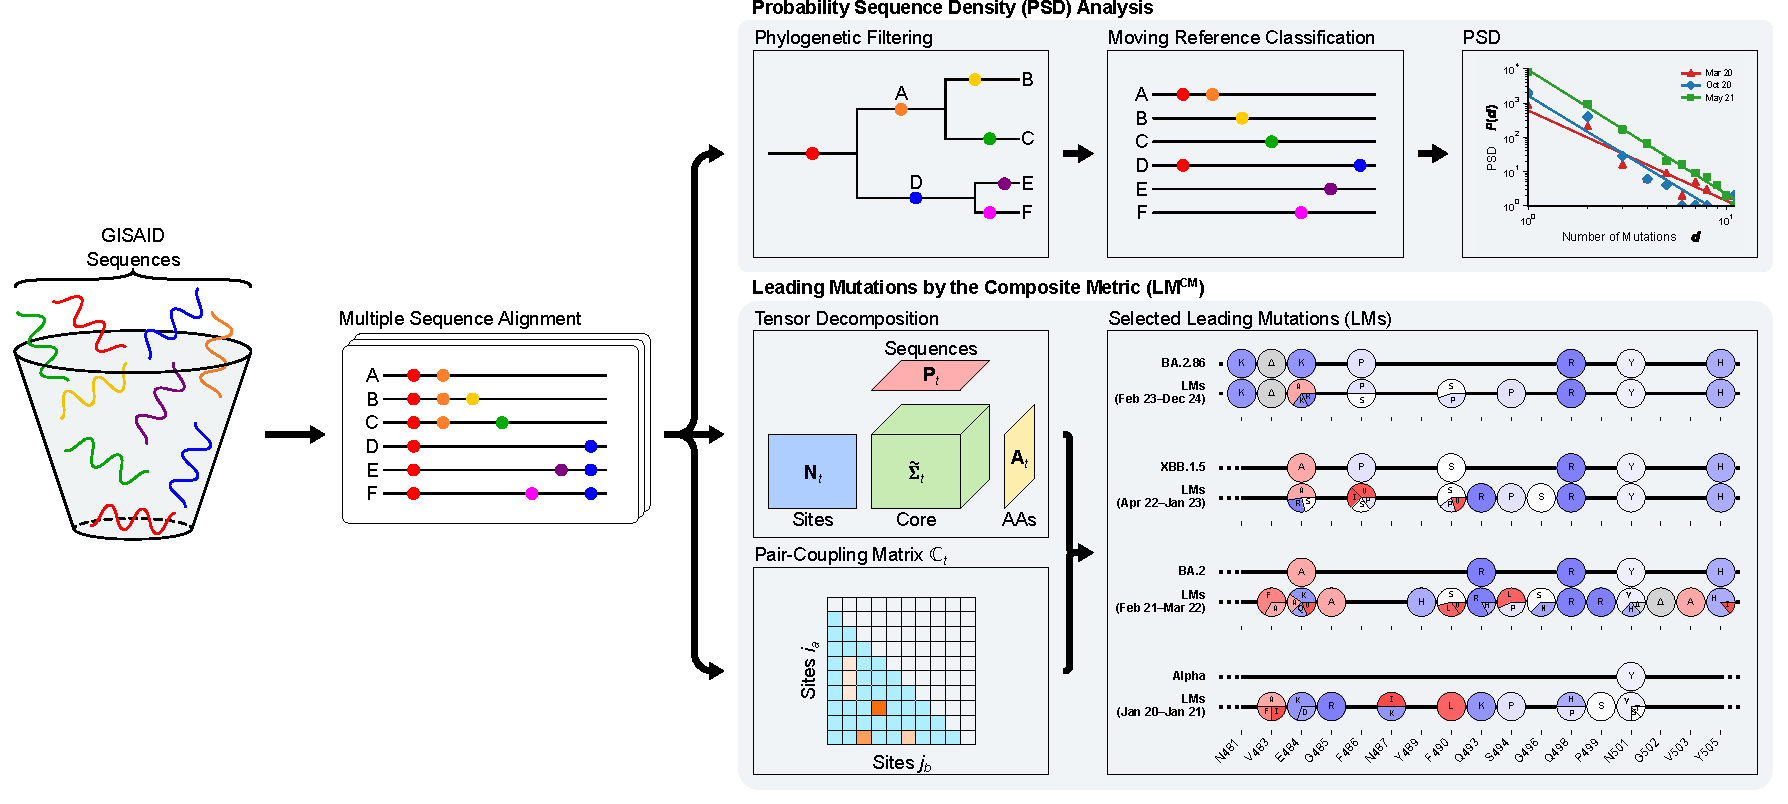
\includegraphics[width=1.\linewidth, angle=0]{Figures/Fig1_Overview+LMCM_new.pdf}
    \caption{A statistical pipeline for deciphering the temporal mutation pattern of the SARS-CoV-2 spike glycoprotein. First, spike glycoprotein amino acid sequences downloaded from the Global Initiative on Sharing All Influenza Data (GISAID) hCoV-19 database are filtered and aligned to generate sets of non-degenerate sequences grouped by month. Then, these data sets are processed in two parallel steps. For the probability sequence density (PSD) $P(\bm{\mathit{d}})$ analysis, the $\log{P(\bm{\mathit{d}})}$-$\log{\bm{\mathit{d}}}$ slope of each monthly data set is computed, and its time gradient can serve as an early warning signal for the emergence of new variants. On the other hand, our leading mutations by the composite metric (LM\textsuperscript{CM}) method integrates sequence, site, and amino acid (AA) data from Tucker decomposition of a mutation tensor, and pair correlation information of mutations, to outline a set of evolutionarily important mutations every month. The diagram of selected leading mutations (LMs) displays a subset of top LMs outlined across four intervals, juxtaposed with the reported mutations carried by representative variants that emerged by the end of each period. Circles or wedges colored blue correspond to mutations that increase hydrophilicity, whereas those colored red indicate the opposite effect. The complete set of LMs outlined each month can be found in Fig.\,S1.}
    \label{Methods}
\end{figure*}

% Another collective feature determined by the emergence of multiple mutations is the statistics of their distributions. Time-resolved analysis of the mutation distributions in viruses allows our understanding of their evolutionary dynamics to be deepened. By incorporating phylogenetic methods, variant clusters can be identified from large-scale sequence datasets, through which the mutation distance between a given progeny and its nearest ancestor can be established \cite{10.1093/ve/veab064, Hadfield2018}. This approach enables the characterization of scaling behaviors in viral evolution --- relationships that quantitatively capture the principles governing the organization and dynamics of complex biological systems \cite{Brown2002, 10.1242/jeb.01589, Newman01092005}. These scaling relationships can be applied to study connections between mutation diversity and genetic distance in the evolution of SARS-CoV-2 spike sequences. While a thorough understanding of both the mutation rate and distribution of SARS-CoV-2 paints a global picture of its evolution, it remains essential to study the details of its amino acid mutations.

% To streamline the process of analyzing all these important characteristics of viral evolution, we previously proposed a method to score the evolutionary significance of mutable sites based on their individual mutation strengths, such that a representative set of key mutations can be identified from endless combinations \cite{Hasan2024}. However, as the spike continues to acquire mutations in large numbers, accounting for their epistatic interactions has become necessary to clarify its evolution \cite{Starr2022Science}.

% Here, we introduce a bifurcated statistical pipeline for deciphering the temporal mutation pattern of the SARS-CoV-2 spike glycoprotein (Fig.\,\ref{Methods}). First, spike glycoprotein amino acid sequences downloaded from the GISAID hCoV-19 database are filtered and aligned to generate sets of non-degenerate sequences grouped by month \cite{cdc_gisaid}. These data sets are then processed in two parallel steps. Our \textit{probability sequence density} (PSD) $P(\mathit{d})$ analysis characterizes the scaling behaviors in viral evolution --- relationships that quantitatively capture the principles governing the organization and dynamics of complex systems \cite{Newman01092005}. In this process, $\log{P(\mathit{d})}$-$\log{\mathit{d}}$ slope of each monthly data set is computed, and its time gradient can serve as an early warning signal for variant emergence. On the other hand, our \textit{leading mutations by the composite metric} (LM\textsuperscript{CM}) method integrates sequence, site, and amino acid data from Tucker decomposition of a mutation tensor, and pair correlation information of mutations, to outline a set of evolutionarily important mutations, coined \textit{leading mutations}, every month. Each set of LM\textsuperscript{CM}-derived leading mutations is publicly accessible on our online platform at \href{https://hbsulab.github.io/deLemus/}{https://hbsulab.github.io/deLemus/}. From these results, we present a comprehensive analysis of the evolutionary dynamics of the SARS-CoV-2 spike glycoprotein by studying temporal heterogeneities within its mutation patterns, shedding light on key mutation trends of the spike glycoprotein.

\section{Numerical Methods}\label{sec:Methods}

% \section{Methodology}

% \subsection{Data Acquisition and Pre-processing}

To elucidate the emergent evolutionary dynamics of the SARS-CoV-2 spike glycoprotein, we implemented a bifurcated statistical pipeline that integrates global scaling analysis with higher-order mutation interaction modeling (Fig.\,\ref{Methods}). Treating viral populations as many-body systems in which mutations interact in a network-like manner, we first applied \textit{probability sequence density} (PSD) analysis, $P(\bm{\mathit{d}})$, to characterize scaling behaviors and monitor temporal changes in the $\log{P(\bm{\mathit{d}})}$-$\bm{\mathit{d}}$ slope as an indicator of evolutionary regime shifts. Complementarily, to account for epistatic interactions among rapidly accumulating mutations, we constructed monthly mutation tensors from multiple sequence alignments and performed Tucker decomposition to extract dominant latent features. These tensor-derived mutation strengths were then integrated with pair-coupling correlations through a composite metric to identify \textit{leading mutations} on a monthly basis.

To track the evolutionary trajectory of the SARS-CoV-2 spike glycoprotein, we compiled a longitudinal dataset spanning four years of the pandemic. By December 2023, more than 15 million amino acid sequences were retrieved from the GISAID hCoV-19 database \cite{gisaid}. We employed the EPI\_ISL\_402124 sequence as the baseline reference for alignment \cite{Zhou2020}. To isolate distinct evolutionary signals and minimize computational redundancy, we implemented a rigorous filtering protocol to remove degenerate (identical) sequences. This resulted in a refined dataset of $667,213$ non-degenerate sequences for analysis.

Sequences were partitioned into temporal cohorts based on their submission month. We applied multiple sequence alignment (MSA) using Clustal Omega \cite{10.1038/msb.2011.75} and assigned phylogenetic lineages using the Nextstrain framework \cite{Hadfield2018}. To distinguish novel evolutionary events from baseline noise, we identified substitutions and deletions by comparing each sequence to its most recent common ancestor.

% \subsection{Quantifying Mutational Dynamics and Scaling}
The primary metric for evolutionary velocity in this study is the sublineage-dependent sequence mutation rate, $\Xi$, reported in units of $\overline{\text{aa}}\, \text{seq}^{-1}\, \text{mo}^{-1}$. To ensure statistical rigor, we calculated the mean mutation rates and their corresponding 95\% confidence intervals (CI) for each major variant, utilizing a Student’s $t$-distribution to account for sample variance.

Furthermore, we investigated the global distribution of mutations through a probability sequence density analysis, $P(\bm{\mathit{d}})$, where $\bm{\mathit{d}}$ represents the number of novel mutated sites across each sequence. By examining the relationship between $P(\bm{\mathit{d}})$ and $\bm{\mathit{d}}$ in a log-log coordinate system, we identified a persistent scaling relationship. The slope of this scaling—derived from the $\log{P(\bm{\mathit{d}})}$-$\log{\bm{\mathit{d}}}$ relationship—was monitored monthly to detect shifts in the virus's evolutionary regime.

% \subsection{Multidimensional Mutation Analysis via Tensor Decomposition}
To capture the complex interdependencies between mutation sites and amino acid types, we represented the MSA data as a high-dimensional mutation tensor. For each month $t$, we constructed an $m \times l \times a_0$ tensor $\widetilde{\mathbf{H}}_t = \big(H_t^{ijk}\big)$, where $m$ is the number of non-degenerate sequences, $l$ is the sequence length (1273 sites), and $a_0$ is the number of amino acid variants (including deletions). An entry $H_t^{ijk} = 1$ signifies the presence of mutation $k$ at site $j$ in sequence $i$.

We decomposed this high-dimensional structure using Tucker decomposition to extract latent features:
\begin{equation}
    \widetilde{\mathbf{H}}_t = \mathbf{P}_t \otimes \widetilde{\mathbf{\Sigma}}_t \otimes \mathbf{N}_t \otimes \mathbf{A}_t,
\end{equation}
where $\mathbf{P}_t$, $\mathbf{N}_t$, and $\mathbf{A}_t$ represent the characteristic matrices for sequences, sites, and amino acid types, respectively. The core tensor $\widetilde{\mathbf{\Sigma}}_t$ contains the weight coefficients (eigenvalues) for these interactions. From these components, we derived a mutation strength matrix $\mathbf{M}_t$, which identifies which amino acid substitutions at specific sites exert the strongest influence on the overall sequence divergence.

% \subsection{The Composite Metric ($LM^{CM}$) Framework}
Evolutionary success is often driven by cooperative mutations rather than isolated events. To quantify these dependencies, we constructed a pair-coupling matrix $\mathbf{C}_t = \big(C_t^{ij}\big)$ based on the correlation of mutation frequencies:
\begin{equation}
    C_t^{ij} = {\left[\sum_{a,b}{\left(f_{t}^{i_{a}j_{b}} - \ f_{t}^{i_{a}}f_{t}^{j_{b}}\right)}\right]}^{1/2},
\end{equation}
where $f_{t}^{i_{a}j_{b}}$ and $f_{t}^{i_{a}}$ denote the joint and marginal frequencies of mutations. Through Singular Value Decomposition (SVD), we isolated the primary pair-coupling matrix $\mathbb{C}_t$, representing the most significant "cooperation" signals between mutation pairs.

Finally, we proposed the \textit{Leading Mutations by the Composite Metric} (LM\textsuperscript{CM}) framework. This framework ranks mutations based on a composite score $L_t^{i_a}$, which integrates individual mutation strength ($M_t^{i_a}$) with its network of couplings ($\mathbb{C}_t^{i_{a}j_{b}}$):
\begin{equation}
    L_t^{i_a} = M_t^{i_a} \sum_{j,b}{\mathbb{C}_t^{i_{a}j_{b}} M_t^{j_b}}.
\end{equation}
By identifying mutations with the highest $L_t^{i_a}$ scores, we can forecast \textit{leading mutations} that are biophysically primed for selection in future variants. This dynamic ranking is updated monthly and served via our open-access platform (\href{https://hbsulab.github.io/deLemus/}{https://hbsulab.github.io/deLemus/}) to assist the global research community in early variant detection.

% To decipher SARS-CoV-2 spike glycoprotein evolution, it is necessary to first compile a dataset of spike sequences. By the end of 2023, we had downloaded more than 15 million SARS-CoV-2 spike glycoprotein amino acid sequences from the GISAID hCoV-19 database \cite{gisaid}, wherein EPI\_ISL\_402124 was selected as the reference sequence \cite{Zhou2020}. Since the original data contained a substantial number of repeated sequences, all degenerate sequences were removed before further analysis of sequence mutations. In total, $667,213$ non-degenerate sequences were retrieved from the entire set of reported sequences uploaded to GISAID between January 2020 and December 2023.

% Sequences submitted to GISAID within the same month were grouped together. Multiple sequence alignment was then applied to each group using Clustal Omega \cite{10.1038/msb.2011.75}. Phylogenetic assignment of sequences to named global outbreak lineages and sublineage annotation were performed using Nextstrain \cite{Hadfield2018}. To clarify mutation patterns in the sequence space, we differentiated novel substitutions or deletions from the inherited ones at each amino acid site by comparing the sequences to their genetically closest ancestors. Based on the total number of mutations per sequence per month for each lineage, the sublineage-dependent sequence mutation rate $\Xi$ was calculated in the unit of $\overline{\text{aa}}\, \text{seq}^{-1}\, \text{mo}^{-1}$. The total number of single amino acid polymorphisms at each $j$\textsuperscript{th} amino acid site in each $t$\textsuperscript{th} month $\bm{\mathit{s}}_j(t)$ and the number of amino acid sites $N(\bm{\mathit{s}})$ were also calculated. From these, a Poisson distribution was observed, giving the monthly average number of amino acid polymorphisms $\bm{\mathit{\overline{s}}}$. The results from Nextstrain also yielded the total number of novel mutated sites $\bm{\mathit{d}}$ across each sequence, and the probability sequence density $P(\bm{\mathit{d}})$, in each month. A persistent scaling relationship between $P(\bm{\mathit{d}})$ and $\bm{\mathit{d}}$ was observed throughout the 48-month period, from which the corresponding $\log{P(\bm{\mathit{d}})}$-$\log{\bm{\mathit{d}}}$ slope was calculated for each month.

% For each $t$\textsuperscript{th} month, one $m\times l \times a_0$ mutation tensor $\widetilde{\mathbf{H}}_t = \big(H_t^{ijk}\big)$ was constructed based on the multiple sequence alignment data, where $m$ is the number of non-degenerate sequences in said month, $l$ is the length of the spike glycoprotein amino acid sequence, and $a_0$ is the number of different amino acid types including deletions. In other words, each slice of the tensor represents one non-degenerate sequence, and each column and row of the slice correspond to the amino acid site and type of that sequence respectively. For the $i$\textsuperscript{th} sequence, if a mutation to the $k$\textsuperscript{th} amino acid type was detected at the $j$\textsuperscript{th} site, then we set $H_t^{ijk} = 1$. Otherwise, $H_t^{ijk} = 0$.

% We then factorized $\widetilde{\mathbf{H}}_t$ by Tucker decomposition:
% \begin{equation}
%     \widetilde{\mathbf{H}}_t = \mathbf{P}_t \otimes \widetilde{\mathbf{\Sigma}}_t \otimes \mathbf{N}_t \otimes \mathbf{A}_t,
% \end{equation}
% where $\mathbf{P}_t$ is an $m\times m$ matrix, $\mathbf{N}_t$ is an $l\times l$ matrix, and $\mathbf{A}_t$ is an $a_0\times a_0$ matrix. $\mathbf{P}_t$, $\mathbf{N}_t$, and $\mathbf{A}_t$ each contains the eigenvector information of the sequence, site, and amino acid type, and their eigenvalues are recorded in the tensor $\widetilde{\mathbf{\Sigma}}_t$. From these components, we defined the special matrix $\mathbf{M}_t$ as the tensor product between $\mathbf{N}_t$ and $\mathbf{A}_t$ weighted by their corresponding eigenvalues in $\widetilde{\mathbf{\Sigma}}_t$, whose element represents the mutation strength of an amino acid at a particular site.

% Additionally, we quantified the correlative effects between mutations by constructing an $n\times n$ pair-coupling matrix $\mathbf{C}_t = \big(C_t^{ij}\big)$ from $\widetilde{\mathbf{H}}_t$, defined as
% \begin{equation}
%     C_t^{ij} = {\left[\sum_{a,b}{\left(f_{t}^{i_{a}j_{b}} - \ f_{t}^{i_{a}}f_{t}^{j_{b}}\right)}\right]}^{1/2},
% \end{equation}
% where $f_{t}^{i_{a}}$ is the frequency of non-degenerate sequences with amino acid $a$ at their $i$\textsuperscript{th} site in the $t$\textsuperscript{th} month, and $f_{t}^{i_{a}j_{b}}$ is that with amino acids $a$ and $b$ at the $i$\textsuperscript{th} and $j$\textsuperscript{th} sites respectively.

% Next, we characterized leading correlations by performing singular value decomposition on $\mathbf{C}_t$:
% \begin{equation}
%     \mathbf{C}_t = \mathbf{W}_t \odot \mathbf{\Sigma}_t \odot {\mathbf{W}_t}^{-1},
% \end{equation}
% where $\mathbf{W}_t$ is a matrix containing cooperation information between mutations and $\mathbf{\Sigma}_t$ is a matrix recording its eigenvalues. By taking the leading elements of $\mathbf{\Sigma}_t$ and $\mathbf{W}_t$, we constructed the primary pair-coupling matrix $\mathbb{C}_t$ to represent the key correlative effects between mutation pairs.

% By combining the single mutation signals and correlative effects encoded in $\mathbf{M}_t$ and $\mathbb{C}_t$ respectively, we propose a composite metric $L_t^{i_a}$ that measures the mutation strength of an amino acid $a$ at the $i$\textsuperscript{th} site, defined by
% \begin{equation}
%     L_t^{i_a} = M_t^{i_a} \sum_{j,b}{\mathbb{C}_t^{i_{a}j_{b}} M_t^{j_b}}.
% \end{equation}
% In particular, $M_t^{i_a}$ refers to the mutation strength of the amino acid $i_a$, and $\mathbb{C}_t^{i_{a}j_{b}}$ denotes the coupling strength between amino acids $i_a$ and $j_b$.

% Using the composite metric $L_t^{i_a}$ associated with each amino acid $i_a$ in the spike glycoprotein, we identify the most evolutionarily significant mutations for every $t$\textsuperscript{th} month; the highest-ranking mutations are designated as \textit{leading mutations}. We term this framework \textit{leading mutations by the composite metric} (LM\textsuperscript{CM}). The set of LM\textsuperscript{CM} selections is dynamically updated on our publicly accessible platform at \href{https://hbsulab.github.io/deLemus/}{https://hbsulab.github.io/deLemus/} to reflect emerging evolutionary trends. Designed specifically for tracking spike evolution, any leading mutations that appear in future SARS-CoV-2 variants would be promptly highlighted on the platform.

\section{Results and Discussion}\label{sec:Results&Discussion}

\subsection{Temporal Dynamics of Mutation Rates}

Mutations are the primary drivers of viral evolution. To understand how novel SARS-CoV-2 variants persistently emerge, it is necessary to decipher the underlying rate at which new mutations appear on its spike glycoprotein \cite{10.1038/s41579-023-00878-2}. For instance, previous studies have reported a negative correlation between the substitutional mutation rate and effective population size of cellular organisms, which is posited by the drift-barrier hypothesis \cite{LYNCH2010345, Lynch2016}. To see if similar relationships can be observed within the diverse SARS-CoV-2 population, we analyzed the behavior of spike mutation rates across its sublineages.

We observed an increase in the sequence-level mutation rate $\Xi$ of the spike glycoprotein over the course of the pandemic (Fig.\,\ref{MutRate}). Early pre-Omicron variants demonstrated relatively low and stable mutation rates, with mean values for D614G ($1.18 \pm 0.05$ $\overline{\text{aa}}\, \text{seq}^{-1}\, \text{mo}^{-1}$) and Alpha ($1.18 \pm 0.09$ $\overline{\text{aa}}\, \text{seq}^{-1}\, \text{mo}^{-1}$) highlighting the limited sequence divergence at the onset of viral transmission \cite{10.1093/ve/veaa061}. Subsequent variants of the Omicron family exhibited elevated $\Xi$ values, with mean rates ranging from $1.41 \pm 0.26$ $\overline{\text{aa}}\, \text{seq}^{-1}\, \text{mo}^{-1}$ for BA.4\&5 to $1.55 \pm 0.47$ $\overline{\text{aa}}\, \text{seq}^{-1}\, \text{mo}^{-1}$ for BA.1, indicative of accelerated evolutionary dynamics and increased mutational variance.

Furthermore, we observed a robust positive correlation between the site-specific mutation rates and the genetic diversity of major SARS-CoV-2 variants. These include B.1.1.7 (Alpha, $\alpha$), B.1.351 (Beta, $\beta$), P.1 (Gamma, $\gamma$), B.1.617.2 (Delta, $\delta$), and Omicron ($o$) (Fig.\,\ref{MutRate} \textbf{Inset}). Direct frequency-based analyses are often susceptible to sampling biases, and certain sequences can be either heavily underrepresented or overrepresented due to discrepancies in sequencing intensities \cite{bias1, bias2}. Using non-degenerate sequence counts therefore serves as a practical analog for effective population size in the context of viral evolution \cite{Wilke2005, 10.1371/journal.pgen.1008271}, reflecting the number of genetically distinct variants that determines the rate at which genetic diversity changes in the population \cite{10.1093/jhered/esac023, https://doi.org/10.1111/mec.17670}. By precisely including each unique sequence exactly once, overrepresentation of frequently sampled sequences in GISAID could be mitigated.

Notably, highly transmissible variants like Delta and Omicron exhibited higher site mutation rates of 0.29 $\overline{\text{aa}}\, \text{site}^{-1}\, \text{mo}^{-1}$ and 0.47 $\overline{\text{aa}}\, \text{site}^{-1}\, \text{mo}^{-1}$ respectively, as well as greater within-variant genetic diversity \cite{Mlcochova2021, Fan2022}. Positive coupling between these traits is expected but mechanistically and causally nontrivial. One interpretation is that a high substitution rate helps maintain genetic diversity within a viral population, which promotes adaptation to optimize its fitness characteristics such as transmissibility \cite{Vignuzzi2006, XIAO2016493}. On the other hand, more transmissible variants could lead to greater generational turnover and thus greater substitution rate and genetic diversity via rapid parallel infection of the host population \cite{10.1093/molbev/msh109}. In contrast, the geographically constrained Beta and Gamma variants displayed comparatively lower site mutation rates and genetic diversities \cite{TEGALLY20233277}.

\begin{figure}[!htbp]
    \centering
    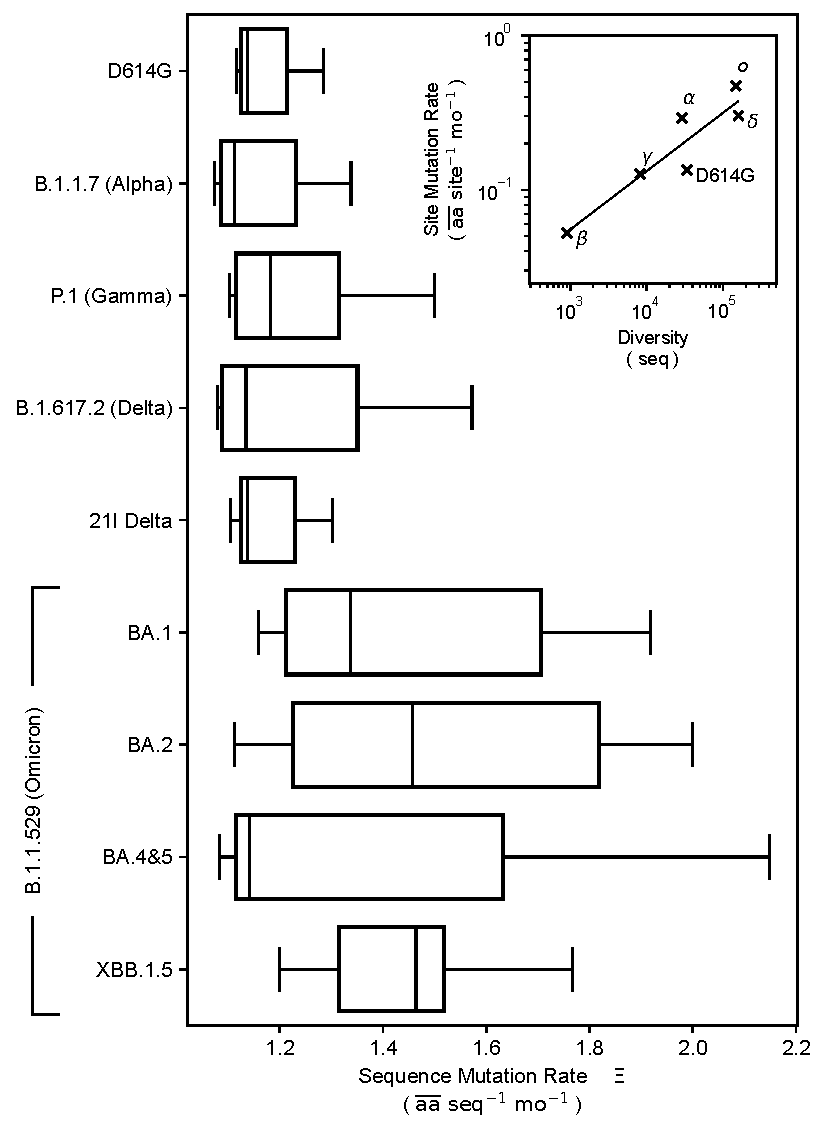
\includegraphics[width= 1.0 \linewidth, angle=0]{Figures/Fig2_MutRate.pdf}
    \caption{Mutation rates $\Xi$ of SARS-CoV-2 spike glycoproteins across major variants, expressed in units of $\overline{\text{aa}}\, \text{seq}^{-1}\, \text{mo}^{-1}$. Variants are ordered top to bottom according to their designation date by the World Health Organization \cite{whoCOVID19Variants}. \textbf{Inset}. Correlation between site mutation rates and effective population size for variants of concern ($R^2 = 0.853$, $n = 6$, 95\% CI $[0.287,0.999]$), expressed in $\overline{\text{aa}}\, \text{site}^{-1}\, \text{mo}^{-1}$. Other abbreviations: $\alpha$ -- B.1.1.7 (Alpha), $\beta$ -- B.1.351 (Beta), $\gamma$ -- P.1 (Gamma), $\delta$ -- B.1.617.2 (Delta), $o$ -- Omicron.} \label{MutRate}
\end{figure}

% Recent studies have suggested that such a burst of mutations equips these saltation variants with enhanced immune evasion capabilities and transmissibility, which may have prompted their global predominance, despite them exhibiting a lower binding affinity to the human angiotensin-converting enzyme 2 (hACE2) than previous strains \cite{WANG202481, Planas2024}.

% Additionally, we revealed a strong positive correlation between site mutation rates and genetic diversity, measured by non-degenerate sequence counts, in SARS-CoV-2 variants of concern (Fig.\,\ref{MutRate}, Inset). As highly transmissible variants like B.1.617.2 (Delta, $\delta$) and Omicron ($o$) have been shown to replicate more rapidly \cite{Mlcochova2021, Fan2022}, they were able to harbor broader mutational spectra, which amplified their site mutation rates ranging from approximately 0.29 to 0.47 $\overline{\text{aa}}\, \text{site}^{-1}\, \text{mo}^{-1}$. In contrast, the B.1.351 (Beta, $\beta$) strain's limited geographic reach reduced its replication opportunities, and consequently its ability to accumulate mutations \cite{Chen2022}. These findings suggest that spike mutations driving transmissibility and infectivity may also enhance the virus's ability to gain mutations by elevating its replication frequency, and hence its diversity.

\subsection{Evolution in the Sequence Space}

Complementing the temporal aspect of viral evolution in terms of rate heterogeneity is the spatial information embedded in its sequence space. To uncover the patterns hidden within such a vast ensemble of sequences, we focused on the scaling behaviors of spike mutations. The use of these statistical relationships may seem otiose at first, but scaling between physical parameters often encapsulates the key underlying organization and dynamics of phenomena in complex systems, particularly in the field of evolutionary biology \cite{SOLE1999156, Brown2002, 10.1242/jeb.01589, Yule1925}. In this study, we defined the term \textit{probability sequence density} (PSD) $P(\bm{\mathit{d}})$, which denotes a probability distribution over the integral displacement $\bm{\mathit{d}}$ of a given sequence from its nearest ancestor in the sequence space. 

\begin{figure}[!htbp]
    \centering
    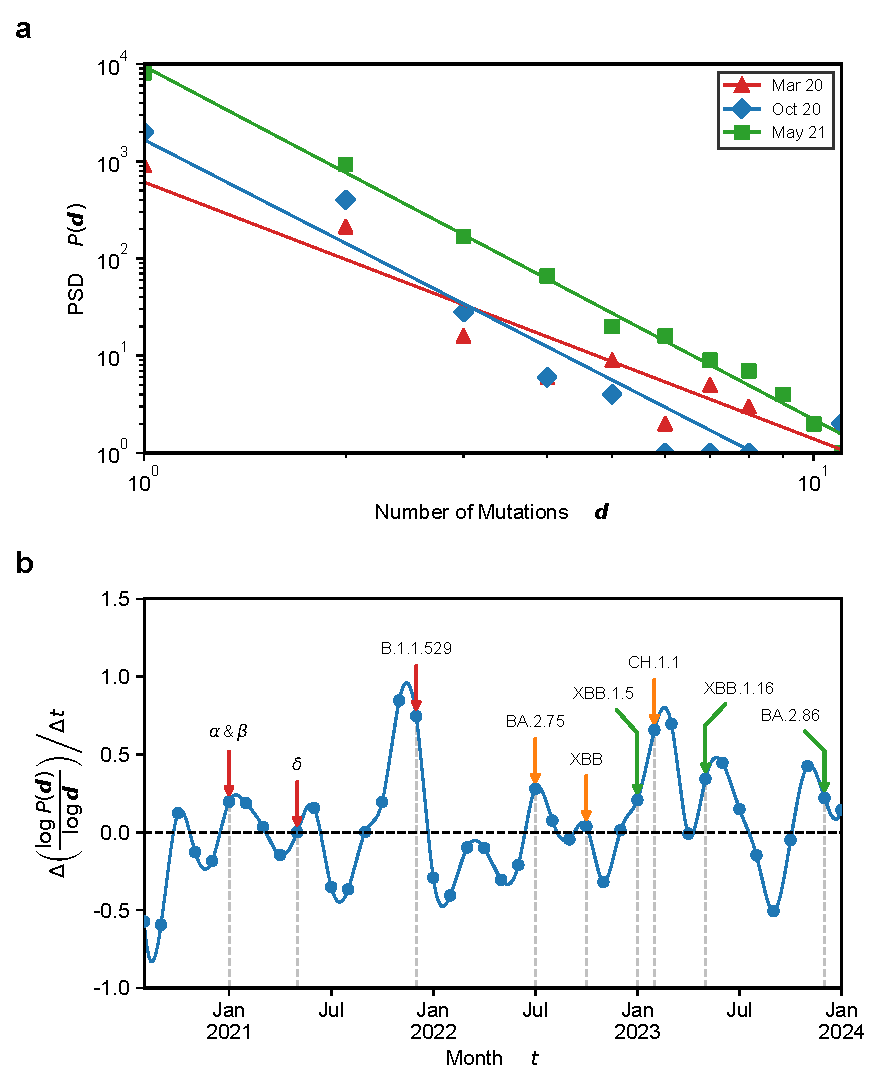
\includegraphics[width=1.0\linewidth]{Figures/Fig3_PSD.pdf}
    \caption{\textbf{a}. Scaling relationship between the probability sequence density (PSD) $P(\mathit{d})$ and number of mutations $\mathit{d}$ in selected months ($R^2_\text{Mar20} = 0.903$ with $n = 10$ and 95\% CI $[0.611, 0.982]$, $R^2_\text{Oct20} = 0.899$ with $n = 9$ and 95\% CI $[0.525, 0.992]$, $R^2_\text{May21} = 0.992$ with $n = 11$ and 95\% CI $[0.967, 0.998]$). \textbf{b}. Evolution of the time gradient $\Delta (\log{P(\mathit{d})} / \log{\mathit{d}}) \big/ \Delta t$. Months wherein notable SARS-CoV-2 strains were designated by the World Health Organization as variants of concern, interest, or under monitoring are annotated with red, green, and orange arrows respectively \cite{whoCOVID19Variants}. Other abbreviations: $\alpha$ -- B.1.1.7 (Alpha), $\beta$ -- B.1.351 (Beta), $\delta$ -- B.1.617.2 (Delta).} \label{Scaling}
\end{figure}

From the PSDs of the monthly non-degenerate sequence sets, we observed a linear scaling relationship between the quantities $P(\bm{\mathit{d}})$ and $\bm{\mathit{d}}$, which manifested itself across different time frames of the SARS-CoV-2 pandemic (Fig.\,\ref{Scaling}\textbf{a}). This scaling was highly robust, and was confirmed by the systematic examination of the $\log{P(\bm{\mathit{d}})}$-$\bm{\mathit{d}}$ plots for every month from January 2020 to December 2023. March 2020, October 2020, and May 2021 were selected as representative snapshots because they illustrate the temporal evolution of the scaling slope during the first major saltation event: transitioning from an early random-mutation regime through the emergence of Alpha and Beta variants and culminating in the rapid global dominance of Delta shortly thereafter \cite{10.1371/journal.pcbi.1010896}.

The effects of this scaling are twofold. First, the consistently negative slope of the $\log{P(\bm{\mathit{d}})}$-$\bm{\mathit{d}}$ plot indicates that spike sequences with lower mutation loads prevailed over those with more mutations in each monthly ensemble. Specifically, most SARS-CoV-2 spike glycoproteins were seen to harbor around one to three mutations per month (Fig.\,\ref{Scaling}\textbf{a}), corroborating previous estimates \cite{Sender2021PNAS}; spike sequences surpassing this range are exceedingly rare. Second, such a scaling relationship can be described as a power law, from which network-like interactions between individual SARS-CoV-2 variants can be inferred \cite{SOLE1999156, Brown2002}. Being a type of heavy-tailed distribution, a power law distribution creates a heightened likelihood of large-valued events than a normal distribution \cite{HALLEY199633, Newman01092005, Yule1925}. This suggests that the evolution of the SARS-CoV-2 spike glycoprotein is a process highly susceptible to abrupt and massive mutational events, likely coming from immunocompromised patients with prolonged infections \cite{10.1056/NEJMsb2104756}. The three major evolutionary leaps sustained by the virus, from Alpha to Delta, from Delta to BA.1, and from XBB to BA.2.86, serve as prime examples that demonstrate how a few extreme events could disproportionately impact the global SARS-CoV-2 population \cite{Viana2022, 10.1371/journal.pcbi.1010896, Planas2024}. Recent studies have suggested that such a burst of mutations equips these saltation variants with enhanced immune evasion capabilities and transmissibility, which may have prompted their global predominance, despite them exhibiting a lower binding affinity to the human angiotensin-converting enzyme 2 (ACE2) than previous strains \cite{WANG202481, Planas2024}.

We further examined the dynamics of the scaling relationships between $P(\bm{\mathit{d}})$ and $\bm{\mathit{d}}$, from which we discovered an intriguing link between the time gradient of the $\log{P(\bm{\mathit{d}})}$-$\log{\bm{\mathit{d}}}$ slope, $\Delta (\log{P(\bm{\mathit{d}})} / \log{\bm{\mathit{d}}}) \big/ \Delta t$, and SARS-CoV-2 spike evolution. In general, $\log{P(\bm{\mathit{d}})} / \log{\bm{\mathit{d}}}$ can be viewed as a quantity describing the shape of the PSD, so its time derivative enables us to track time-dependent changes in the distribution of spike sequences based on their $\bm{\mathit{d}}$ values. For example, a reduction in this ratio corresponds to a shift toward a sequence ensemble dominated by low-$\bm{\mathit{d}}$ sequences, whereas an increment corresponds to the opposite. Under this interpretation, large positive peaks in a $\Delta (\log{P(\bm{\mathit{d}})} / \log{\bm{\mathit{d}}}) \big/ \Delta t$-time plot would represent a sudden influx of heavily mutated spike sequences within the virus population, which would signify the emergence of a new variant. In alignment with our hypothesis, while multiple peaks and troughs can be observed from Fig.\,\ref{Scaling}\textbf{b}, the emergence of most major SARS-CoV-2 variants is accompanied by a positive peak in the time gradient. Therefore, this finding suggests the importance of PSD analysis in understanding the evolution of viruses, showing it can be used for the early detection of variant displacement events.

% Analysis of the monthly non-degenerate sequence sets revealed a consistent power-law scaling between the sequence density $P(\bm{\mathit{d}})$ and the number of amino acid substitutions $\bm{\mathit{d}}$ (Fig.\,\ref{Scaling}A). Most spike protein sequences accumulated between one and three mutations per month, while highly mutated variants were comparatively rare, suggesting evolutionary constraints on spike sequence divergence. To quantify temporal shifts in this evolutionary landscape, we computed the gradient of the log-log slope over time, defined as $\Delta (\log{P(\bm{\mathit{d}})} / \log{\bm{\mathit{d}}}) \big/ \Delta t$. Peaks in this gradient frequently coincided with the emergence of major SARS-CoV-2 lineages (Fig.\,\ref{Scaling}B), indicating bursts of accelerated sequence diversification associated with the rise of new variants.

\subsection{Evolution of Leading Mutations}

\begin{figure*}[!htbp]
    \centering
    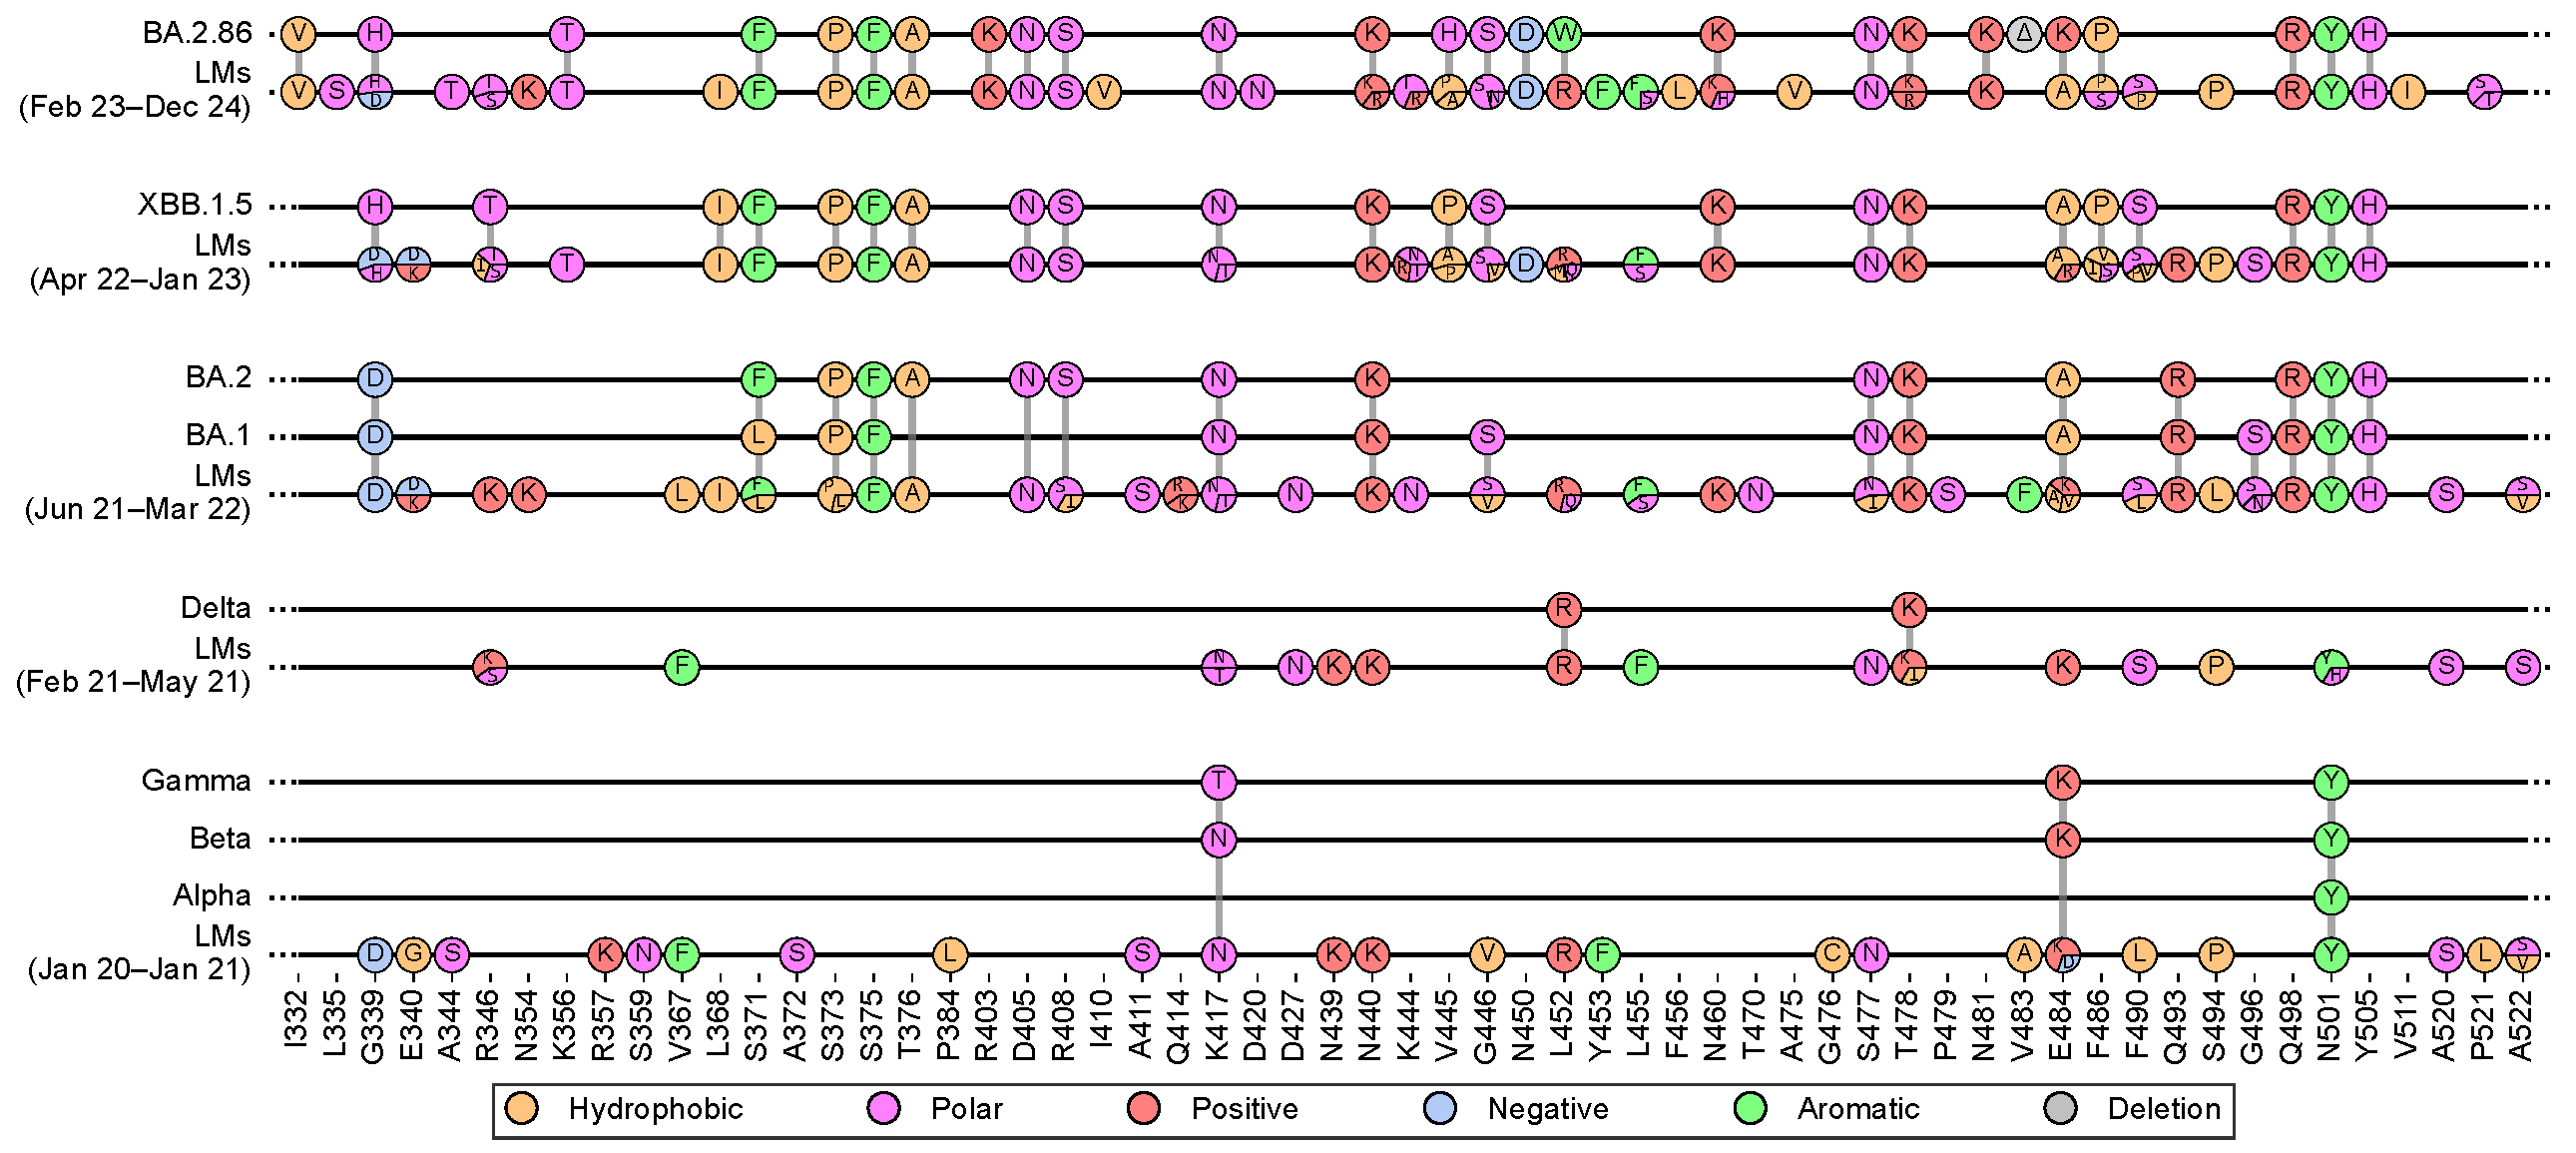
\includegraphics[width=1.0\linewidth]{Figures/Fig4_LMCM_mains.pdf}
    \caption{Top-ranked LM\textsuperscript{CM}-outlined leading mutations (LMs) in the receptor-binding domain (RBD) of the spike. Variants designated as variants of concern or interest in the same month by the World Health Organization are grouped together \cite{whoCOVID19Variants}. Each pie chart represents the distribution of top-ranked LMs for a given month, where each colored sector corresponds to a specific mutation and its relative frequency within that month's top-ranked set. Vertical lines connect LMs with reported mutations if they coincide. The color scheme corresponds to the side-chain property of the residue being mutated to: Hydrophobic (orange; A, I, L, V, G, P, C, M), polar (magenta; H, N, Q, S, T), positive (red; K, R), negative (blue; D, E), aromatic (lime; F, W, Y), and deletion (gray; $\Delta$). The complete set of RBD LMs can be found in Fig.\,S1 and S2.} \label{LMCM}
\end{figure*}

% To characterize how mutations shape the evolutionary trajectory of SARS-CoV-2 in greater detail, we analyzed the mutation patterns of each amino acid site across the spike glycoprotein. Given the large number of existing spike mutations, identifying those that exert the strongest influence on viral evolution is critical. Addressing this challenge, we developed the LM\textsuperscript{CM} method to effectively outline leading mutations in the spike glycoprotein. These leading mutations are tracked and publicly accessible via our online platform at \href{https://hbsulab.github.io/deLemus/}{https://hbsulab.github.io/deLemus/}. To exemplify the evolutionary significance of the LM\textsuperscript{CM}-outlined leading mutations, a representation selection of these located in the receptor-binding domain (RBD) of the spike glycoprotein is displayed in Fig.\,\ref{LMCM}.

% Several key RBD mutations in SARS-CoV-2 have emerged across different variants, significantly impacting ACE2 binding affinity. The N501Y mutation, first identified in June 2020 using the LM\textsuperscript{CM} method, is present in Alpha, Beta, Gamma, Mu, and Omicron variants; it enhances ACE2 interaction through $\pi$-$\pi$ stacking with Y41 of ACE2 \cite{Dejnirattisai2021}. Similarly, the E484K mutation, observed from January 2020 and notably found in the Beta variant, promotes stronger ACE2 binding via local structural rearrangements when combined with N501Y and D614G \cite{Mannar2021}. The T478K mutation, highlighted in November 2020 and characteristic of the Delta variant, facilitates tighter RBD-ACE2 binding by forming additional hydrogen bonds at the interface \cite{10.1038/s41467-022-28528-w}. Another mutation associated with Delta, L452R, was identified in April 2020, and contributes to increased ACE2 affinity through secondary structure rearrangements when part of a triple mutation \cite{10.1039/D1CP04005G}. Finally, the N440K mutation, outlined in the Omicron variant, enhances electrostatic complementarity with ACE2, aiding its high transmissibility.

% The time-resolved spectra of the LM\textsuperscript{CM}-derived leading mutations bridge the gap between the global evolutionary trends in sequence ensembles and local functional alterations in the spike protein caused by individual mutations. One notable trend we observed was the accumulation of basic or polar amino acids in the RBD of the spike (Fig.\,S1). This convergence in physicochemical properties of substitutions was particularly pronounced within the receptor-binding domain (RBM) of the RBD  (Fig.\,S3), an essential stretch of amino acids that engages the hACE2 receptor to mediate viral entry into host cells \cite{Jackson2022}. While the enrichment of positively charged or polar residues in the RBM tends to improve spike-receptor interactions due to the predominantly negatively charged surface of the hACE2 receptor (Fig.\,S4B) \cite{Jawad2021, 10.1002/cbic.202100681}, the convergence ratio --- defined here as the monthly fraction of novel leading mutations among all RBM-based leading mutations --- revealed a plateau in this trend over time (Fig.\,S4A). This saturation may suggest a potential evolutionary trade-off between the charge optimization of the RBM for better infectivity and the immune evasion capability of the virus \cite{10.1093/procel/pwae007}. In fact, recent studies has reported that newer Omicron subvariants exhibit diminishing gains in hACE2-binding affinity when compared to their predecessors \cite{Nguyen2024, Wang31122024}.


To characterize how mutations shape the evolutionary trajectory of SARS-CoV-2 in greater detail, we analyzed the mutation patterns of each amino acid site across the spike glycoprotein. Given the large number of existing spike mutations, identifying those that exert the strongest influence on viral evolution is critical for forecasting future genomic shifts. Addressing this challenge, we developed the LM\textsuperscript{CM} method to effectively outline leading mutations in the spike glycoprotein, providing a predictive window into which residues are likely to drive upcoming variant emergence. These leading mutations are tracked and publicly accessible via our online platform at \href{https://hbsulab.github.io/deLemus/}{https://hbsulab.github.io/deLemus/}. To exemplify the predictive power and evolutionary significance of the LM\textsuperscript{CM}-outlined leading mutations, a representation selection of these located in the receptor-binding domain (RBD) of the spike glycoprotein is displayed in Fig.\,\ref{LMCM}.

Several key RBD mutations in SARS-CoV-2 have emerged across different variants, significantly impacting ACE2 binding affinity; notably, the LM\textsuperscript{CM} method consistently identified these dangerous substitutions months before they achieved global dominance. The N501Y mutation, first identified as a leading mutation in June 2020 using the LM\textsuperscript{CM} method—well before the surge of the Alpha variant—is present in Alpha, Beta, Gamma, Mu, and Omicron variants; it enhances ACE2 interaction through $\pi$-$\pi$ stacking with Y41 of ACE2 \cite{Dejnirattisai2021}. Similarly, the E484K mutation, captured by our model as early as January 2020 and notably found in the Beta variant, promotes stronger ACE2 binding via local structural rearrangements when combined with N501Y and D614G \cite{Mannar2021}. The T478K mutation, highlighted by LM\textsuperscript{CM} in November 2020 as a future mutation of concern and later found characteristic of the Delta variant, facilitates tighter RBD-ACE2 binding by forming additional hydrogen bonds at the interface \cite{10.1038/s41467-022-28528-w}. Another mutation associated with Delta, L452R, was identified by our pipeline in April 2020, and contributes to increased ACE2 affinity through secondary structure rearrangements when part of a triple mutation \cite{10.1039/D1CP04005G}. Finally, the N440K mutation, outlined by LM\textsuperscript{CM} as an evolutionarily significant site, enhances electrostatic complementarity with ACE2, aiding its high transmissibility.

The time-resolved spectra of the LM\textsuperscript{CM}-derived leading mutations bridge the gap between the global evolutionary trends in sequence ensembles and local functional alterations in the spike protein, allowing for the early detection of fitness-enhancing amino acid substitutions. One notable trend we observed was the accumulation of basic or polar amino acids in the RBD of the spike (Fig.\,S1). This convergence in physicochemical properties of substitutions was particularly pronounced within the receptor-binding domain (RBM) of the RBD (Fig.\,S3), an essential stretch of amino acids that engages the hACE2 receptor to mediate viral entry into host cells \cite{Jackson2022}. While the enrichment of positively charged or polar residues in the RBM tends to improve spike-receptor interactions due to the predominantly negatively charged surface of the hACE2 receptor (Fig.\,S4B) \cite{Jawad2021, 10.1002/cbic.202100681}, the convergence ratio --- defined here as the monthly fraction of novel leading mutations among all RBM-based leading mutations --- revealed a plateau in this trend over time (Fig.\,S4A). This saturation, identified through our leading mutation analysis, may suggest a potential evolutionary trade-off between the charge optimization of the RBM for better infectivity and the immune evasion capability of the virus \cite{10.1093/procel/pwae007}. In fact, recent studies have reported that newer Omicron subvariants exhibit diminishing gains in hACE2-binding affinity when compared to their predecessors \cite{Nguyen2024, Wang31122024}, a shift in evolutionary strategy that can be anticipated by monitoring the divergence in LM\textsuperscript{CM} spectral outputs. By identifying these evolutionarily significant sites months before they manifest in dominant global variants, the LM\textsuperscript{CM} framework demonstrates a robust capacity to predict future dangerous mutations, serving as a proactive computational sentinel for anticipating the physicochemical trajectory of viral evolution.


% \section{Discussion}

% Mutations are the primary drivers of viral evolution. To understand how novel SARS-CoV-2 variants persistently emerge, it is necessary to decipher the underlying rate at which new mutations appear on its spike glycoprotein \cite{10.1038/s41579-023-00878-2}. For instance, previous studies have reported a strong negative correlation between the substitutional mutation rate and effective population size of cellular organisms, which is posited by the drift-barrier hypothesis \cite{LYNCH2010345, Lynch2016}.To see if similar relationships can be observed within the diverse SARS-CoV-2 population, we analyzed the behavior of spike mutation rates across its sublineages.

% Our analysis of $\Xi$ revealed a temporal escalation in sequence mutation rates. Initially, the mutation rate remained low and steady due to the limited acquisition of mutations within the pool of early variants \cite{10.1093/ve/veaa061}. The $\Xi$ of variants that emerged thereafter was generally higher compared to that of their predecessors, particularly in variants that achieved widespread transmission. Recent studies have suggested that such a burst of mutations equips these saltation variants with enhanced immune evasion capabilities and transmissibility, which may have prompted their global predominance, despite them exhibiting a lower binding affinity to the human angiotensin-converting enzyme 2 (hACE2) than previous strains \cite{WANG202481, Planas2024}.

% The positive correlation between site mutation rate and effective population size suggests that replication frequency is a key driver of mutational diversity. B.1.617.2 (Delta, $\delta$) and Omicron ($o$) have been shown to replicate more rapidly \cite{Mlcochova2021, Fan2022}, they were able to harbor broader mutational spectra. In contrast, the B.1.351 (Beta, $\beta$) strain's limited geographic reach reduced its replication opportunities, and consequently its ability to accumulate mutations \cite{Chen2022}. These findings suggest that spike mutations driving transmissibility and infectivity may also enhance the virus's ability to gain mutations by elevating its replication frequency, and hence its diversity.

% Complementing the temporal aspect of viral evolution in terms of rate heterogeneity is the spatial information embedded in its sequence space. To uncover the patterns hidden within such a vast ensemble of sequences, we focused on the scaling behaviors of spike mutations. The use of these statistical relationships may seem otiose at first, but scaling between physical parameters often encapsulates the key underlying organization and dynamics of phenomena in complex systems, particularly in the field of evolutionary biology \cite{SOLE1999156, Brown2002, 10.1242/jeb.01589, Yule1925}. In this study, we defined the term \textit{probability sequence density} (PSD) $P(\bm{\mathit{d}})$, which denotes a probability distribution over the integral displacement $\bm{\mathit{d}}$ of a given sequence from its nearest ancestor in the sequence space. 

% From the PSDs of the monthly non-degenerate sequence sets, we observed a linear scaling relationship between the quantities $P(\bm{\mathit{d}})$ and $\bm{\mathit{d}}$, which manifested itself across different time frames of the SARS-CoV-2 pandemic (Fig.\,\ref{Scaling}A). The effects of this scaling are twofold. First, the consistently negative slope of the $\log{P(\bm{\mathit{d}})}$-$\bm{\mathit{d}}$ plot indicates that spike sequences with lower mutation loads prevailed over those with more mutations in each monthly ensemble. Specifically, most SARS-CoV-2 spike glycoproteins were seen to harbor around one to three mutations per month (Fig.\,\ref{Scaling}A), corroborating previous estimates \cite{Sender2021PNAS}; spike sequences surpassing this range are exceedingly rare. Second, such a scaling relationship can be described as a power law, from which network-like interactions between individual SARS-CoV-2 variants can be inferred \cite{SOLE1999156, Brown2002}. Being a type of heavy-tailed distribution, a power law distribution creates a heightened likelihood of large-valued events than a normal distribution \cite{HALLEY199633, Newman01092005, Yule1925}. This suggests that the evolution of the SARS-CoV-2 spike glycoprotein is a process highly susceptible to abrupt and massive mutational events. The two major evolutionary leaps sustained by the virus, from Delta to BA.1, and from XBB to BA.2.86, serve as prime examples that demonstrate how a few extreme events could disproportionately impact the global SARS-CoV-2 population \cite{Viana2022, Planas2024}.

% We further examined the dynamics of the scaling relationships between $P(\bm{\mathit{d}})$ and $\bm{\mathit{d}}$, from which we discovered an intriguing link between the time gradient of the $\log{P(\bm{\mathit{d}})}$-$\log{\bm{\mathit{d}}}$ slope, $\Delta (\log{P(\bm{\mathit{d}})} / \log{\bm{\mathit{d}}}) \big/ \Delta t$, and SARS-CoV-2 spike evolution. In general, $\log{P(\bm{\mathit{d}})} / \log{\bm{\mathit{d}}}$ can be viewed as a quantity describing the shape of the PSD, so its time derivative enables us to track time-dependent changes in the distribution of spike sequences based on their $\bm{\mathit{d}}$ values. For example, a reduction in this ratio corresponds to a shift toward a sequence ensemble dominated by low-$\bm{\mathit{d}}$ sequences, whereas an increment corresponds to the opposite. Under this interpretation, large positive peaks in a $\Delta (\log{P(\bm{\mathit{d}})} / \log{\bm{\mathit{d}}}) \big/ \Delta t$-time plot would represent a sudden influx of heavily mutated spike sequences within the virus population, which would signify the emergence of a new variant. In alignment with our hypothesis, while multiple peaks and troughs can be observed from Fig.\,\ref{Scaling}B, the emergence of most major SARS-CoV-2 variants is accompanied by a positive peak in the time gradient. Therefore, this finding suggests the importance of PSD analysis in understanding the evolution of viruses, showing it can be used for the early detection of variant displacement events.

% The time-resolved spectra of the LM\textsuperscript{CM}-derived leading mutations bridge the gap between the global evolutionary trends in sequence ensembles and local functional alterations in the spike protein caused by individual mutations. One notable trend we observed was the accumulation of basic or polar amino acids in the receptor-binding domain (RBD) of the spike (Fig.\,S1). This convergence in physicochemical properties of substitutions was particularly pronounced within the receptor-binding domain (RBM) of the RBD  (Fig.\,S3), an essential stretch of amino acids that engages the hACE2 receptor to mediate viral entry into host cells \cite{Jackson2022}. While the enrichment of positively charged or polar residues in the RBM tends to improve spike-receptor interactions due to the predominantly negatively charged surface of the hACE2 receptor (Fig.\,S4B) \cite{Jawad2021, 10.1002/cbic.202100681}, the convergence ratio --- defined here as the monthly fraction of novel leading mutations among all RBM-based leading mutations --- revealed a plateau in this trend over time (Fig.\,S4A). This saturation may suggest a potential evolutionary trade-off between the charge optimization of the RBM for better infectivity and the immune evasion capability of the virus \cite{10.1093/procel/pwae007}. In fact, recent studies has reported that newer Omicron subvariants exhibit diminishing gains in hACE2-binding affinity when compared to their predecessors \cite{Nguyen2024, Wang31122024}. 

% Collectively, our results underscore the importance of integrating mutation rate dynamics, sequence space scaling, and site-specific mutation impact to understand SARS-CoV-2 evolution. These insights reinforce the utility of platforms like deLemus in tracking and forecasting viral adaptation.

\section{Conclusions}\label{sec:Conclusions}

Our statistical pipeline allowed us to characterize the collective effects arising from the mass acquisition of mutations by the SARS-CoV-2 spike glycoprotein. From our comprehensive analysis, several distinct patterns were revealed in the temporal and spatial domains of its evolution. For the former, mutation rate heterogeneity across variants, exemplified by its increase in recent Omicron sublineages, underscored the virus's capacity to perpetuate its continual adaptation. For the latter, the power-law scaling we uncovered highlights how a very few extreme mutational leaps can entirely reshape the evolutionary trajectory of the virus. In particular, this enabled us to devise the temporal gradient of the $\log{P(\bm{\mathit{d}})}$-$\log{\bm{\mathit{d}}}$ slope, capable of quantifying these abrupt shifts, as an early indicator for the emergence of evolutionarily important variants. Moreover, at the single amino acid level, our LM\textsuperscript{CM} method bridges the global sequence ensemble dynamics with site-specific functional impacts of individual mutations by outlining crucial leading mutations within massive sequence data sets; its results are posted in our publicly accessible platform at \href{https://hbsulab.github.io/deLemus/}{https://hbsulab.github.io/deLemus/}. Overall, the findings advance our understanding of viral evolution and demonstrates the need for extensive disease surveillance to better understand the evolutionary dynamics of circulating viruses.


\begin{acknowledgments}

We acknowledge the data contributors and the GISAID Initiative for sharing the genetic sequences. This work is supported in part by the Research Grants Council of Hong Kong (16305623), HKUST 20-20 Grant (VP2020S25SC04), Guangdong S$\&$T Program (2025A0505000027), and Society of Interdisciplinary Research (SOIRÉE).

\end{acknowledgments}

% \bibliography{reference}% Produces the bibliography via BibTeX.
\printbibliography
\end{document}
%
% ****** End of file apssamp.tex ******
